\chapter{The Large Hadron Collider}
\label{chap:LHC}

The \ac{LHC}~\cite{Evans:2008zzb} is a circular particle physics accelerator located near Geneva, Switzerland. It collides protons at four interaction points, which correspond to the four major experiments hosted by the \ac{LHC}: the \ac{ALICE}~\cite{ALICE:2008ngc}, \ac{ATLAS}~\cite{ATLAS:2008xda}, \ac{CMS}~\cite{CMS:2008xjf}, and \ac{LHCb}~\cite{LHCb:2008vvz} experiments. Accelerating proton beams to TeV-level requires a chain of acceleration stages before they are energetic enough for the final injection into the \ac{LHC} ring. These stages of acceleration and the whole \ac{CERN} accelerator complex are discussed in \autoref{sec:CERN}. The number of collision events delivered by the \ac{LHC} is measured in units called ``luminosity''. The definition of luminosity is discussed in \autoref{sec:Lumi}. The long term schedule for the \ac{LHC} is discussed in \autoref{sec:Plan}.

\section{The CERN Accelerator Complex}
\label{sec:CERN}

Installed in a 27 km circular tunnel previously used for the \ac{LEP} collider~\cite{203828}, the \ac{LHC} is the largest and most powerful particle accelerator ever existed. The primary objective of the \ac{LHC} is to deliver high intensity and high energy proton collisions, allowing physicists to study the laws of nature at the most fundamental scale. This objective is achieved through a complex system of accelerators, which rapidly accelerates protons to the target energy in a multistage process, maintains the proton energy, focuses, and collides them precisely at the designated locations. The full system is illustrated in Figure~\ref{fig:LHC}.

\begin{figure}[tbh!]
 \begin{center}
 \begin{tabular}{c}
 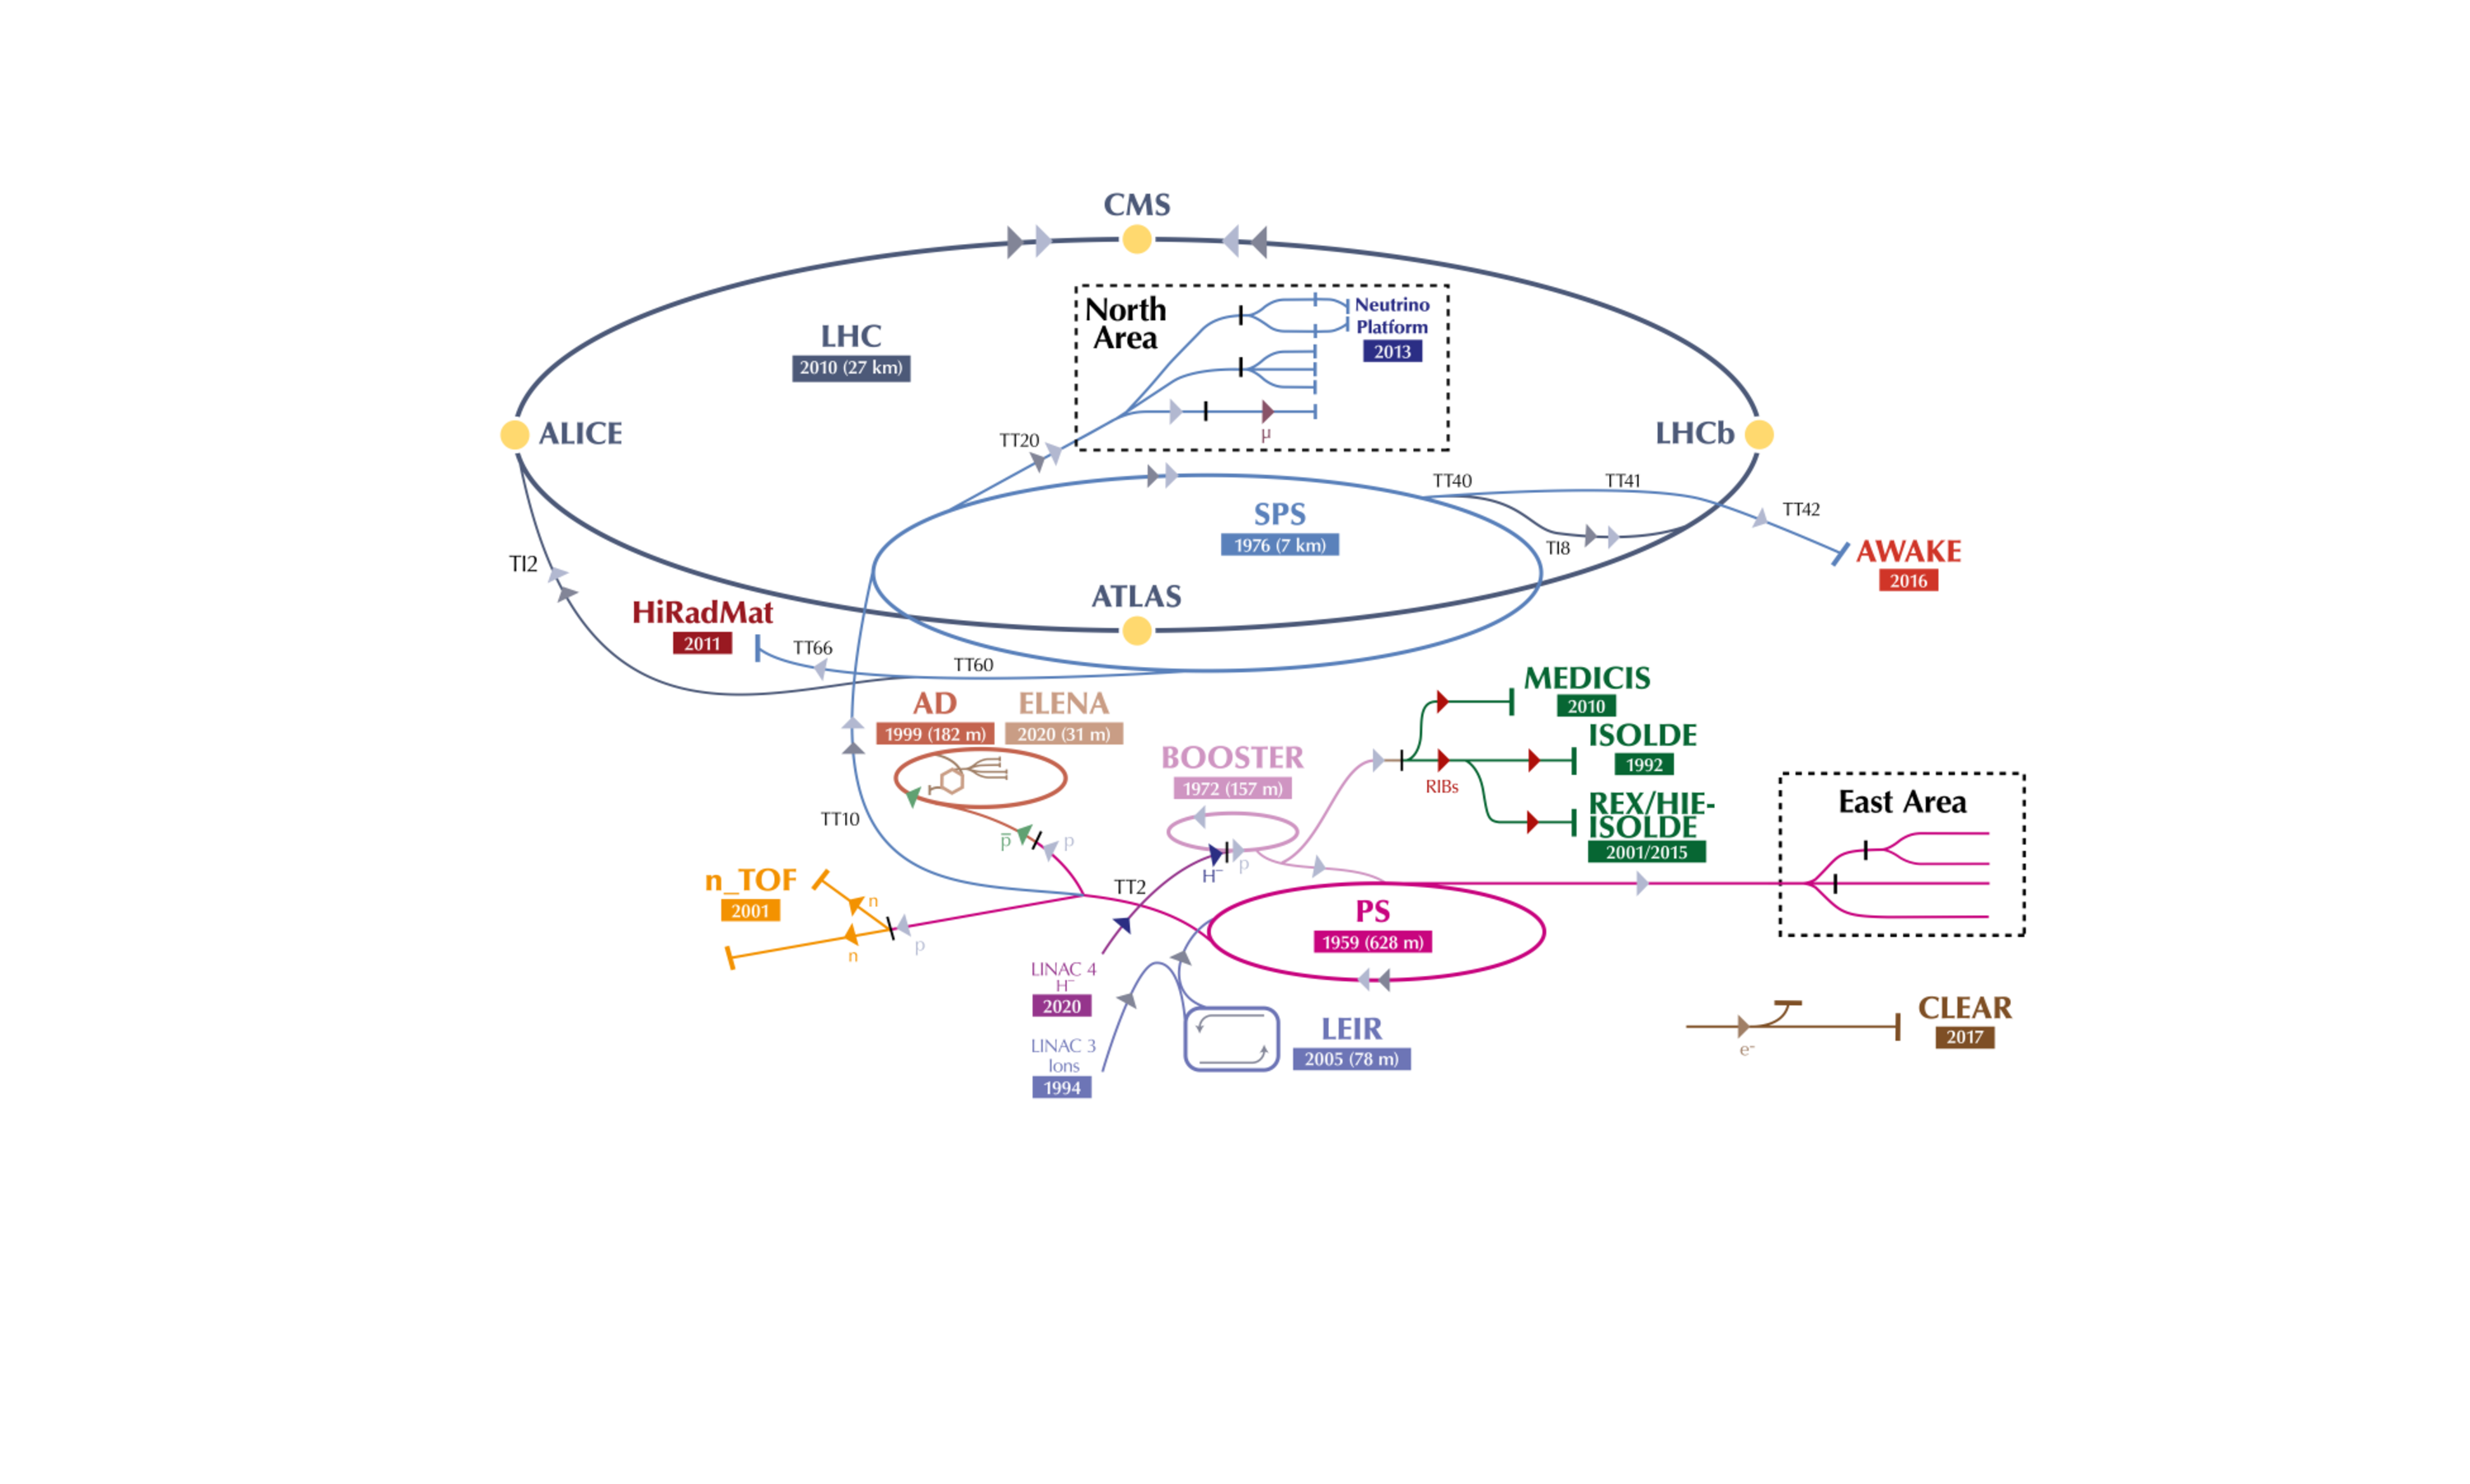
\includegraphics[width=\textwidth]{figures/Part2/LHC/CERN}
 \end{tabular}
 \caption{Layout of the \ac{CERN} accelerator complex, adapted from~\cite{CERN:2022}.}
 \label{fig:LHC}
 \end{center}
\end{figure}

Until 2018, an older linear accelerator (LINAC 2) was used to initially accelerate protons to 50 MeV. After 2018, negative hydrogen ions (H$^{-}$) are accelerated by the Linear accelerator 4 (LINAC 4)~\cite{Vretenar:2020quc} to 160 MeV using cylindrical conductors charged by radiofrequency cavities. Quadrupole magnets are placed along the accelerator to keep the beam focused.  The hydrogen ions are then stripped of their two electrons during injection into the Proton Synchrotron Booster (BOOSTER)~\cite{Reich:1969fw}, which is a circular accelerator that boosts protons to 2 GeV. Protons are then injected into the Proton Synchrotron (PS), which accelerates them to 25 GeV before injecting them into the second largest machine in the accelerator complex called the \ac{SPS}. The \ac{SPS} is a 7 km circular accelerator that uses room-temperature dipole magnets to bend the protons. Protons are accelerated by the \ac{SPS} to an energy of 450 GeV before entering the final accelerator ring -- the \ac{LHC}. The \ac{LHC} uses super-conducting dipole magnets up to 8.4 T to bend protons and ultimately accelerate them to 6.8 TeV during Run-3. Quadrupole magnets are placed at four collision points to focus the proton beams, which eventually collide at the \ac{IP} of each detector. 

\section{Luminosity}
\label{sec:Lumi}

The total number of events of a given process is given by 

\begin{equation}
N=\int\mathcal{L}\sigma dt,
\end{equation}

where $\sigma$ is the cross-section of the process and $\mathcal{L}$ is known as the instantaneous luminosity that can be written in a simplified form

\begin{equation}
\mathcal{L}=\frac{N^2f}{A},
\end{equation}

where $N$ is the total number of protons in each beam, $f$ is the frequency of the beam crossing, and $A$ is the cross-sectional area of the beam crossing.

The \ac{LHC} is designed to deliver an instantaneous luminosity $\mathcal{L}=10^{34}\textsf{cm}^{-2}~\textsf{s}^{-1}$ which corresponds to an event rate of 1 billion collisions per second, assuming the inelastic cross-section $\sigma^{\textsf{pp}}_{\textsf{in}}~=$ 100 mb. The delivered integrated luminosity by year of data taking is shown in Figure~\ref{fig:twikilumi}.

The peak instantaneous luminosity reached $2\times10^{34}~\textsf{cm}^{-2}\textsf{s}^{-1}$ in 2018, which is factor of two larger than the design value of the \ac{LHC}. High instantaneous luminosity means more collision events are delivered by the \ac{LHC}, but it also brings a side effect -- multiple interactions per crossing, also known as \ac{PU} . The average number of \ac{PU} increased from 27 in 2016 to 52 in 2023, creating challenges for data-taking and event reconstruction. The \ac{PU} profile for each year of data taking is shown in \ref{fig:twikilumi}.

\begin{figure}[tbh!]
 \begin{center}
 \begin{tabular}{cc}
 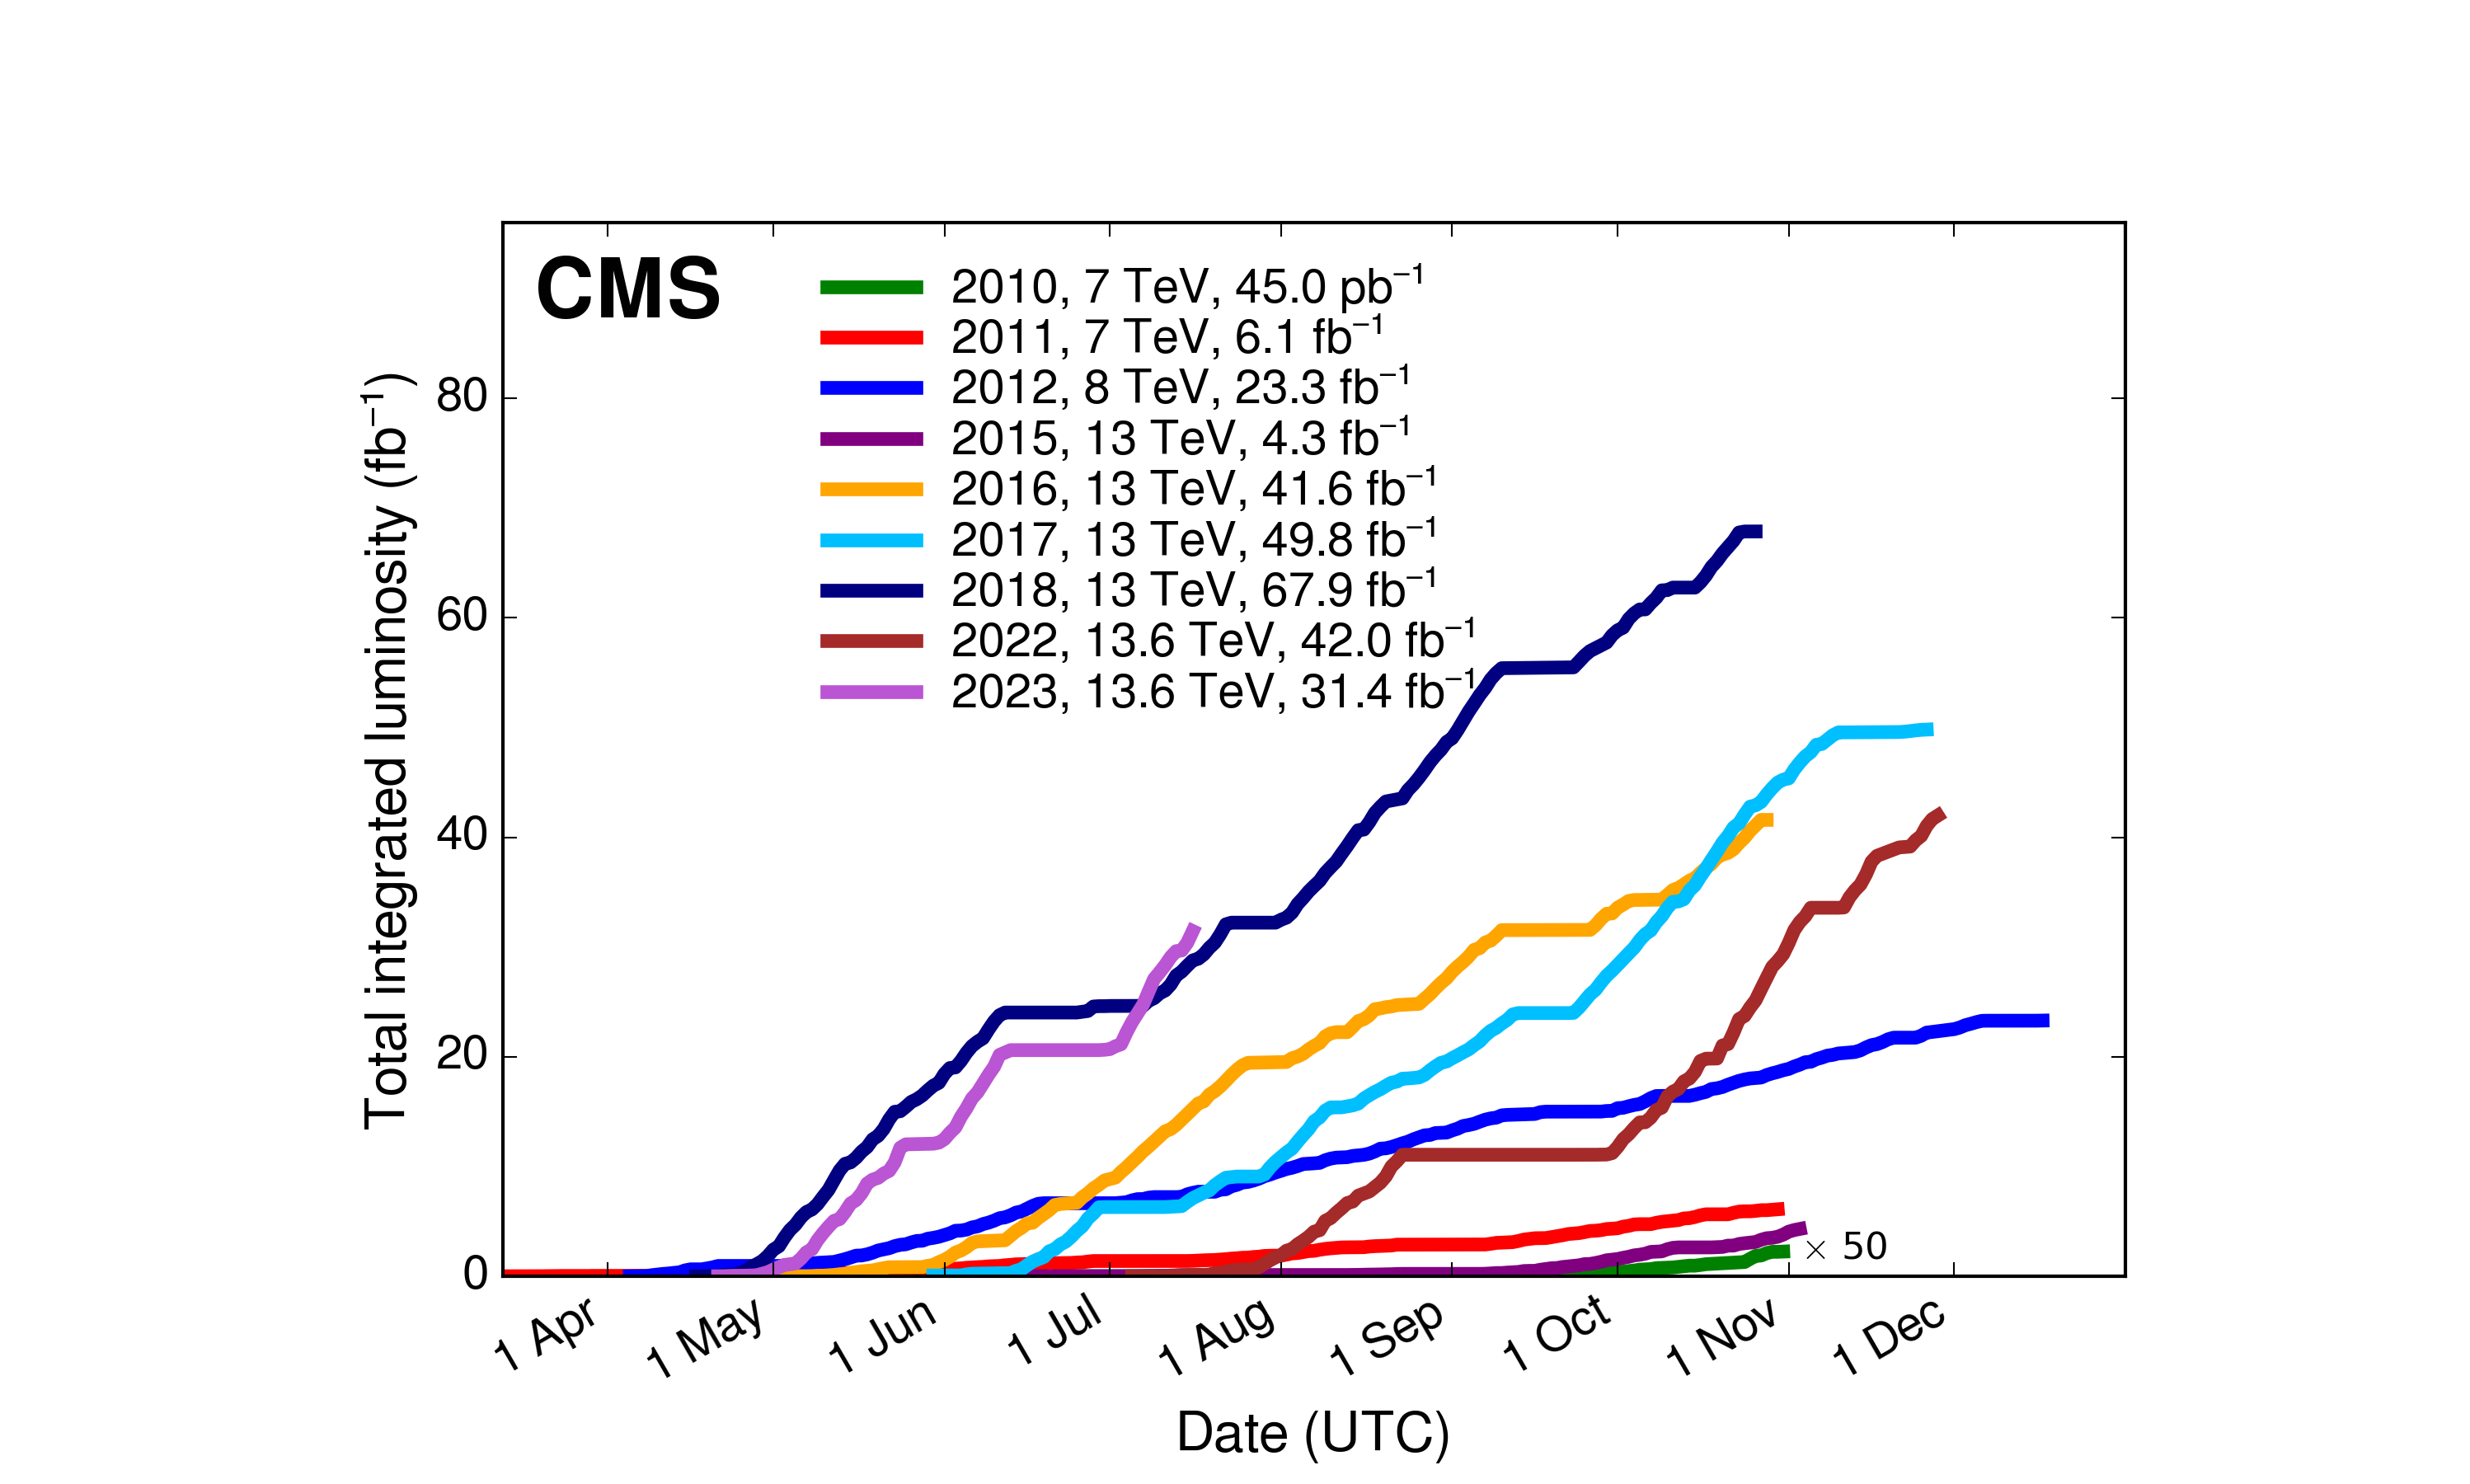
\includegraphics[width=0.48\textwidth]{figures/Part2/LHC/twikilumi}&
 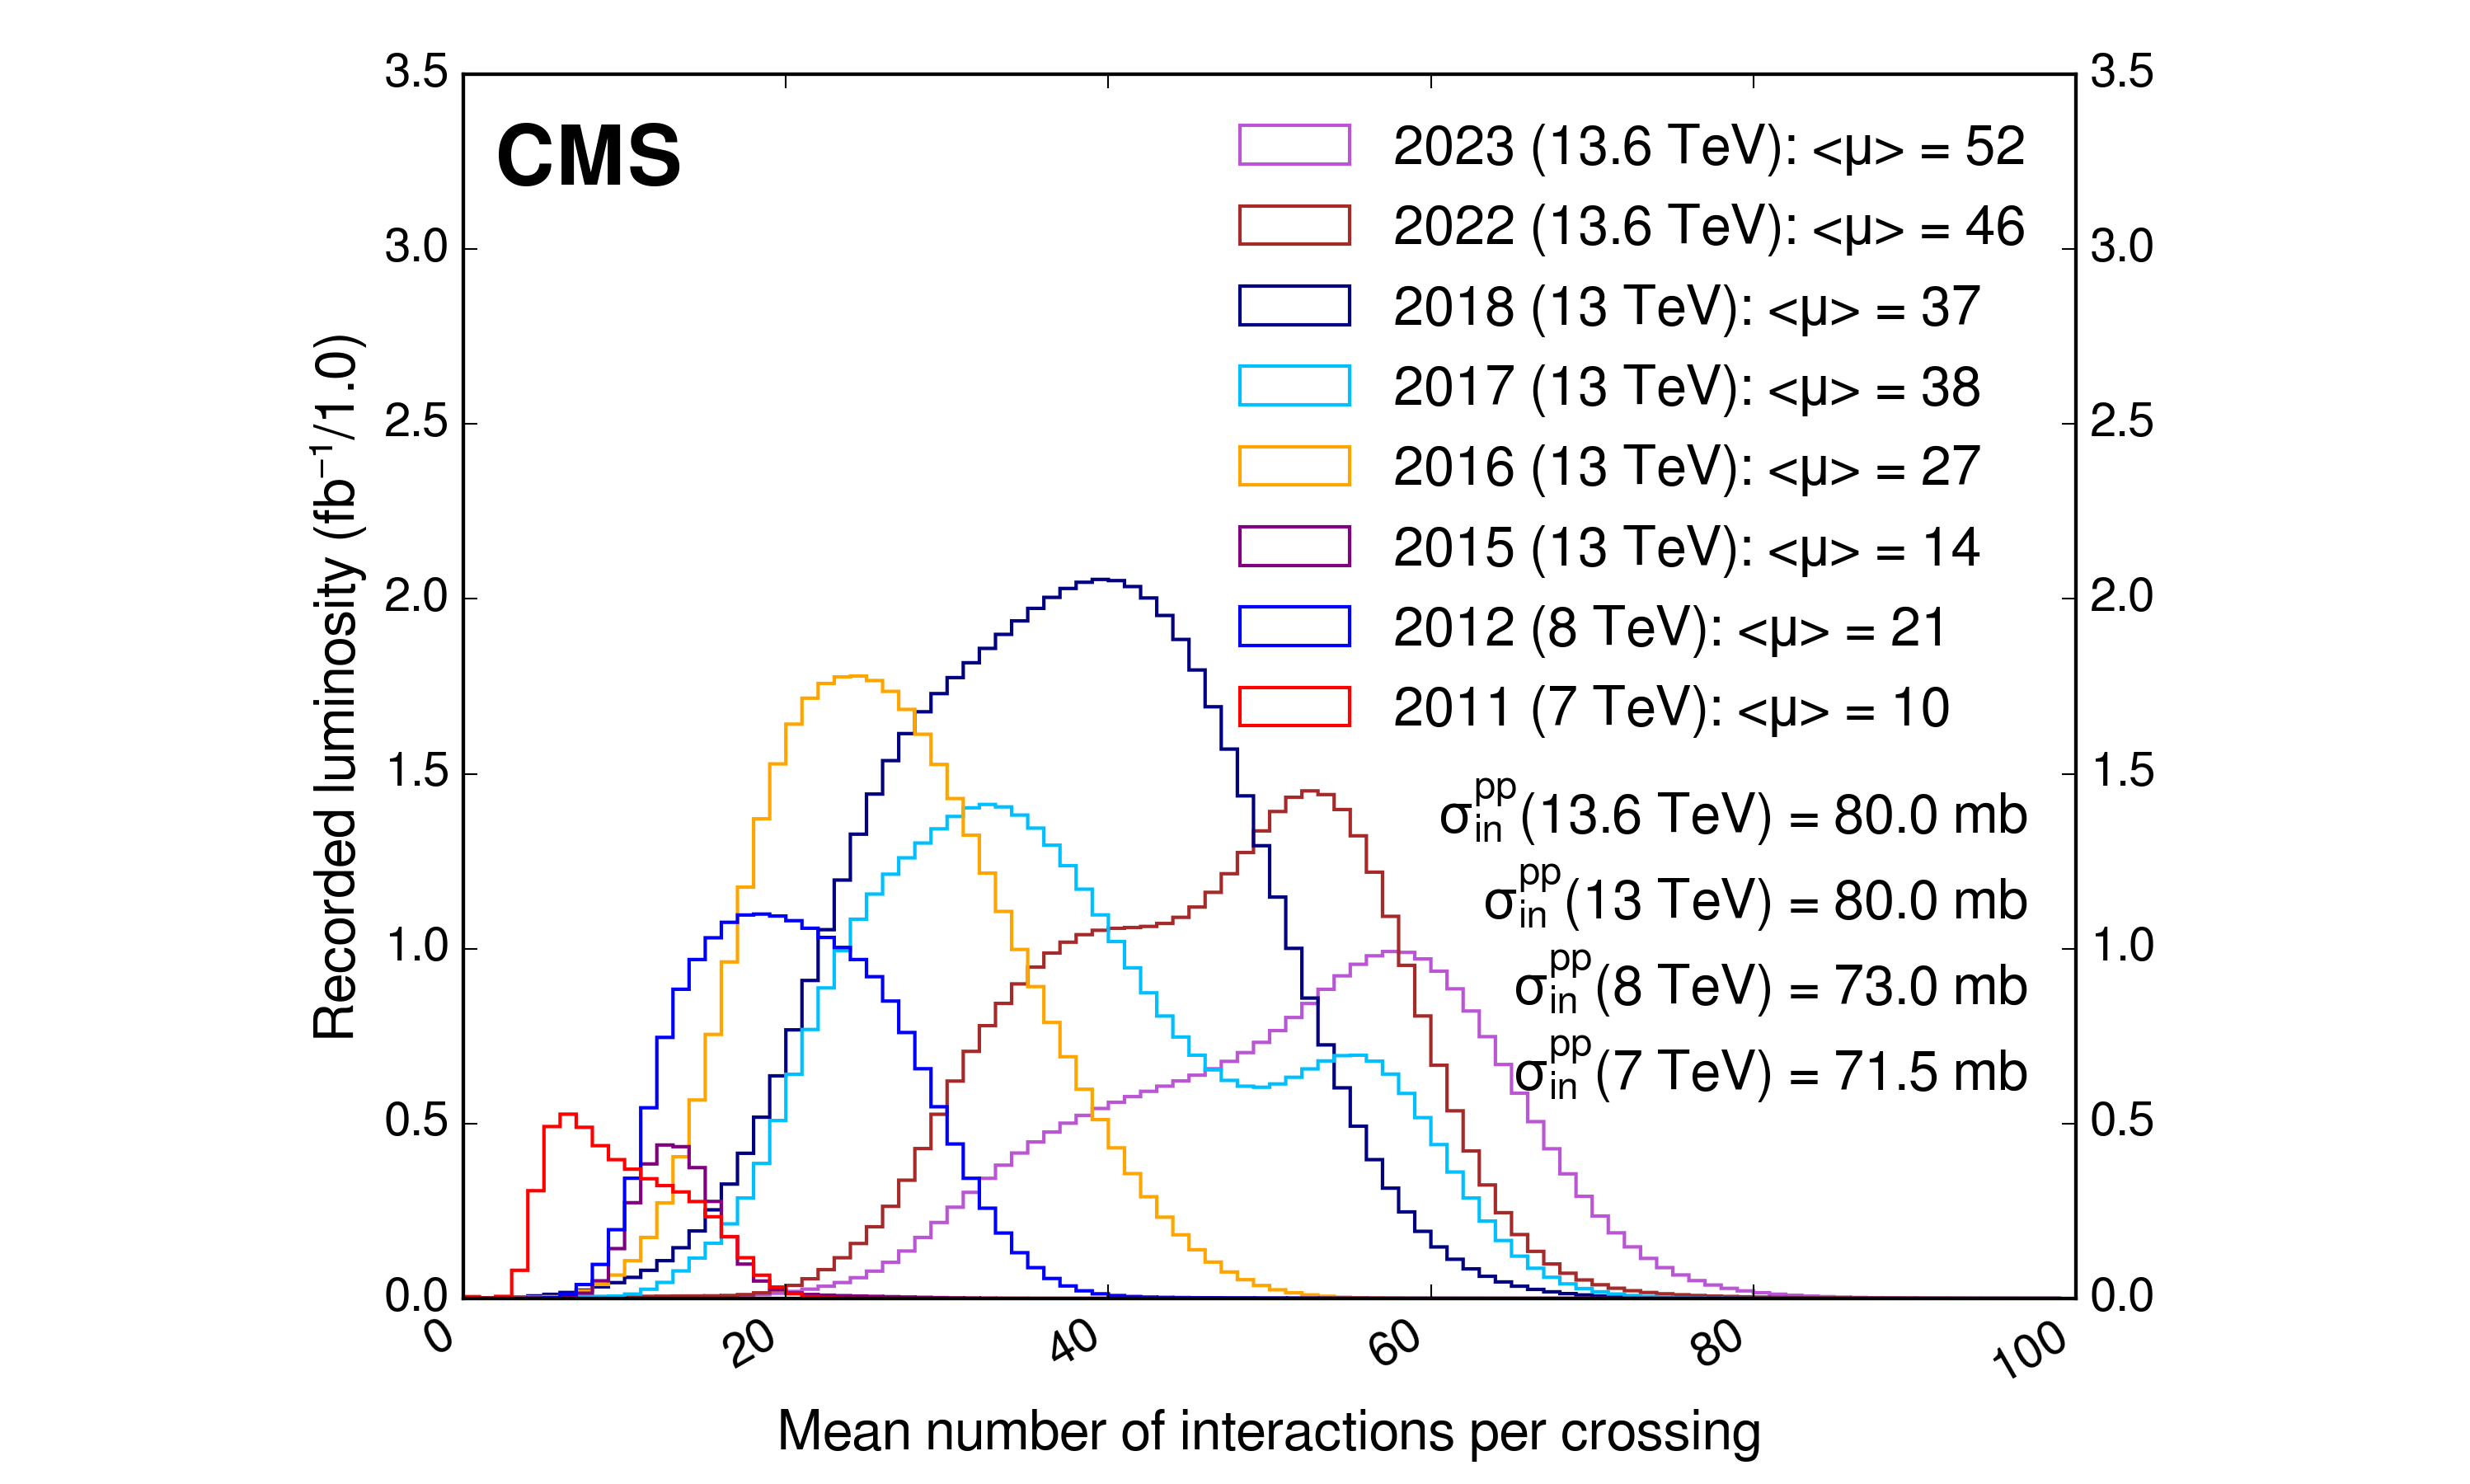
\includegraphics[width=0.48\textwidth]{figures/Part2/LHC/twikipu}\\
 \end{tabular}
 \caption{Delivered integrated luminosity versus time (left) and recorded luminosity versus mean number of interactions per crossing (left), taken from~\cite{twiki:lumi}.}
 \label{fig:twikilumi}
 \end{center}
\end{figure} 

\section{LHC Long Term Schedule}
\label{sec:Plan}

The Long Shutdown 2 (LS2) lasted for over 3 three years until the \ac{LHC} resumed data taking in mid 2022. The on-going run of the \ac{LHC}, known as Run-3, is expected to end in 2025. Between 2026 and 2028 is a period known as the Long Shutdown 3 (LS3), when major upgrades of the \ac{LHC} and the hosted experiments will take place. A new era of the \ac{LHC}, known as the \ac{HL-LHC} will arrive in 2029, when the instantaneous luminosity will gradually increase to up to a factor $7.5$ more than the designed value. The \ac{HL-LHC} is expected to be operational for more than 10 years until the 2040s. A summary of the \ac{LHC} long term schedule is shown in Figure~\ref{fig:Schedule}.

\begin{figure}[tbh!]
 \begin{center}
 \begin{tabular}{c}
 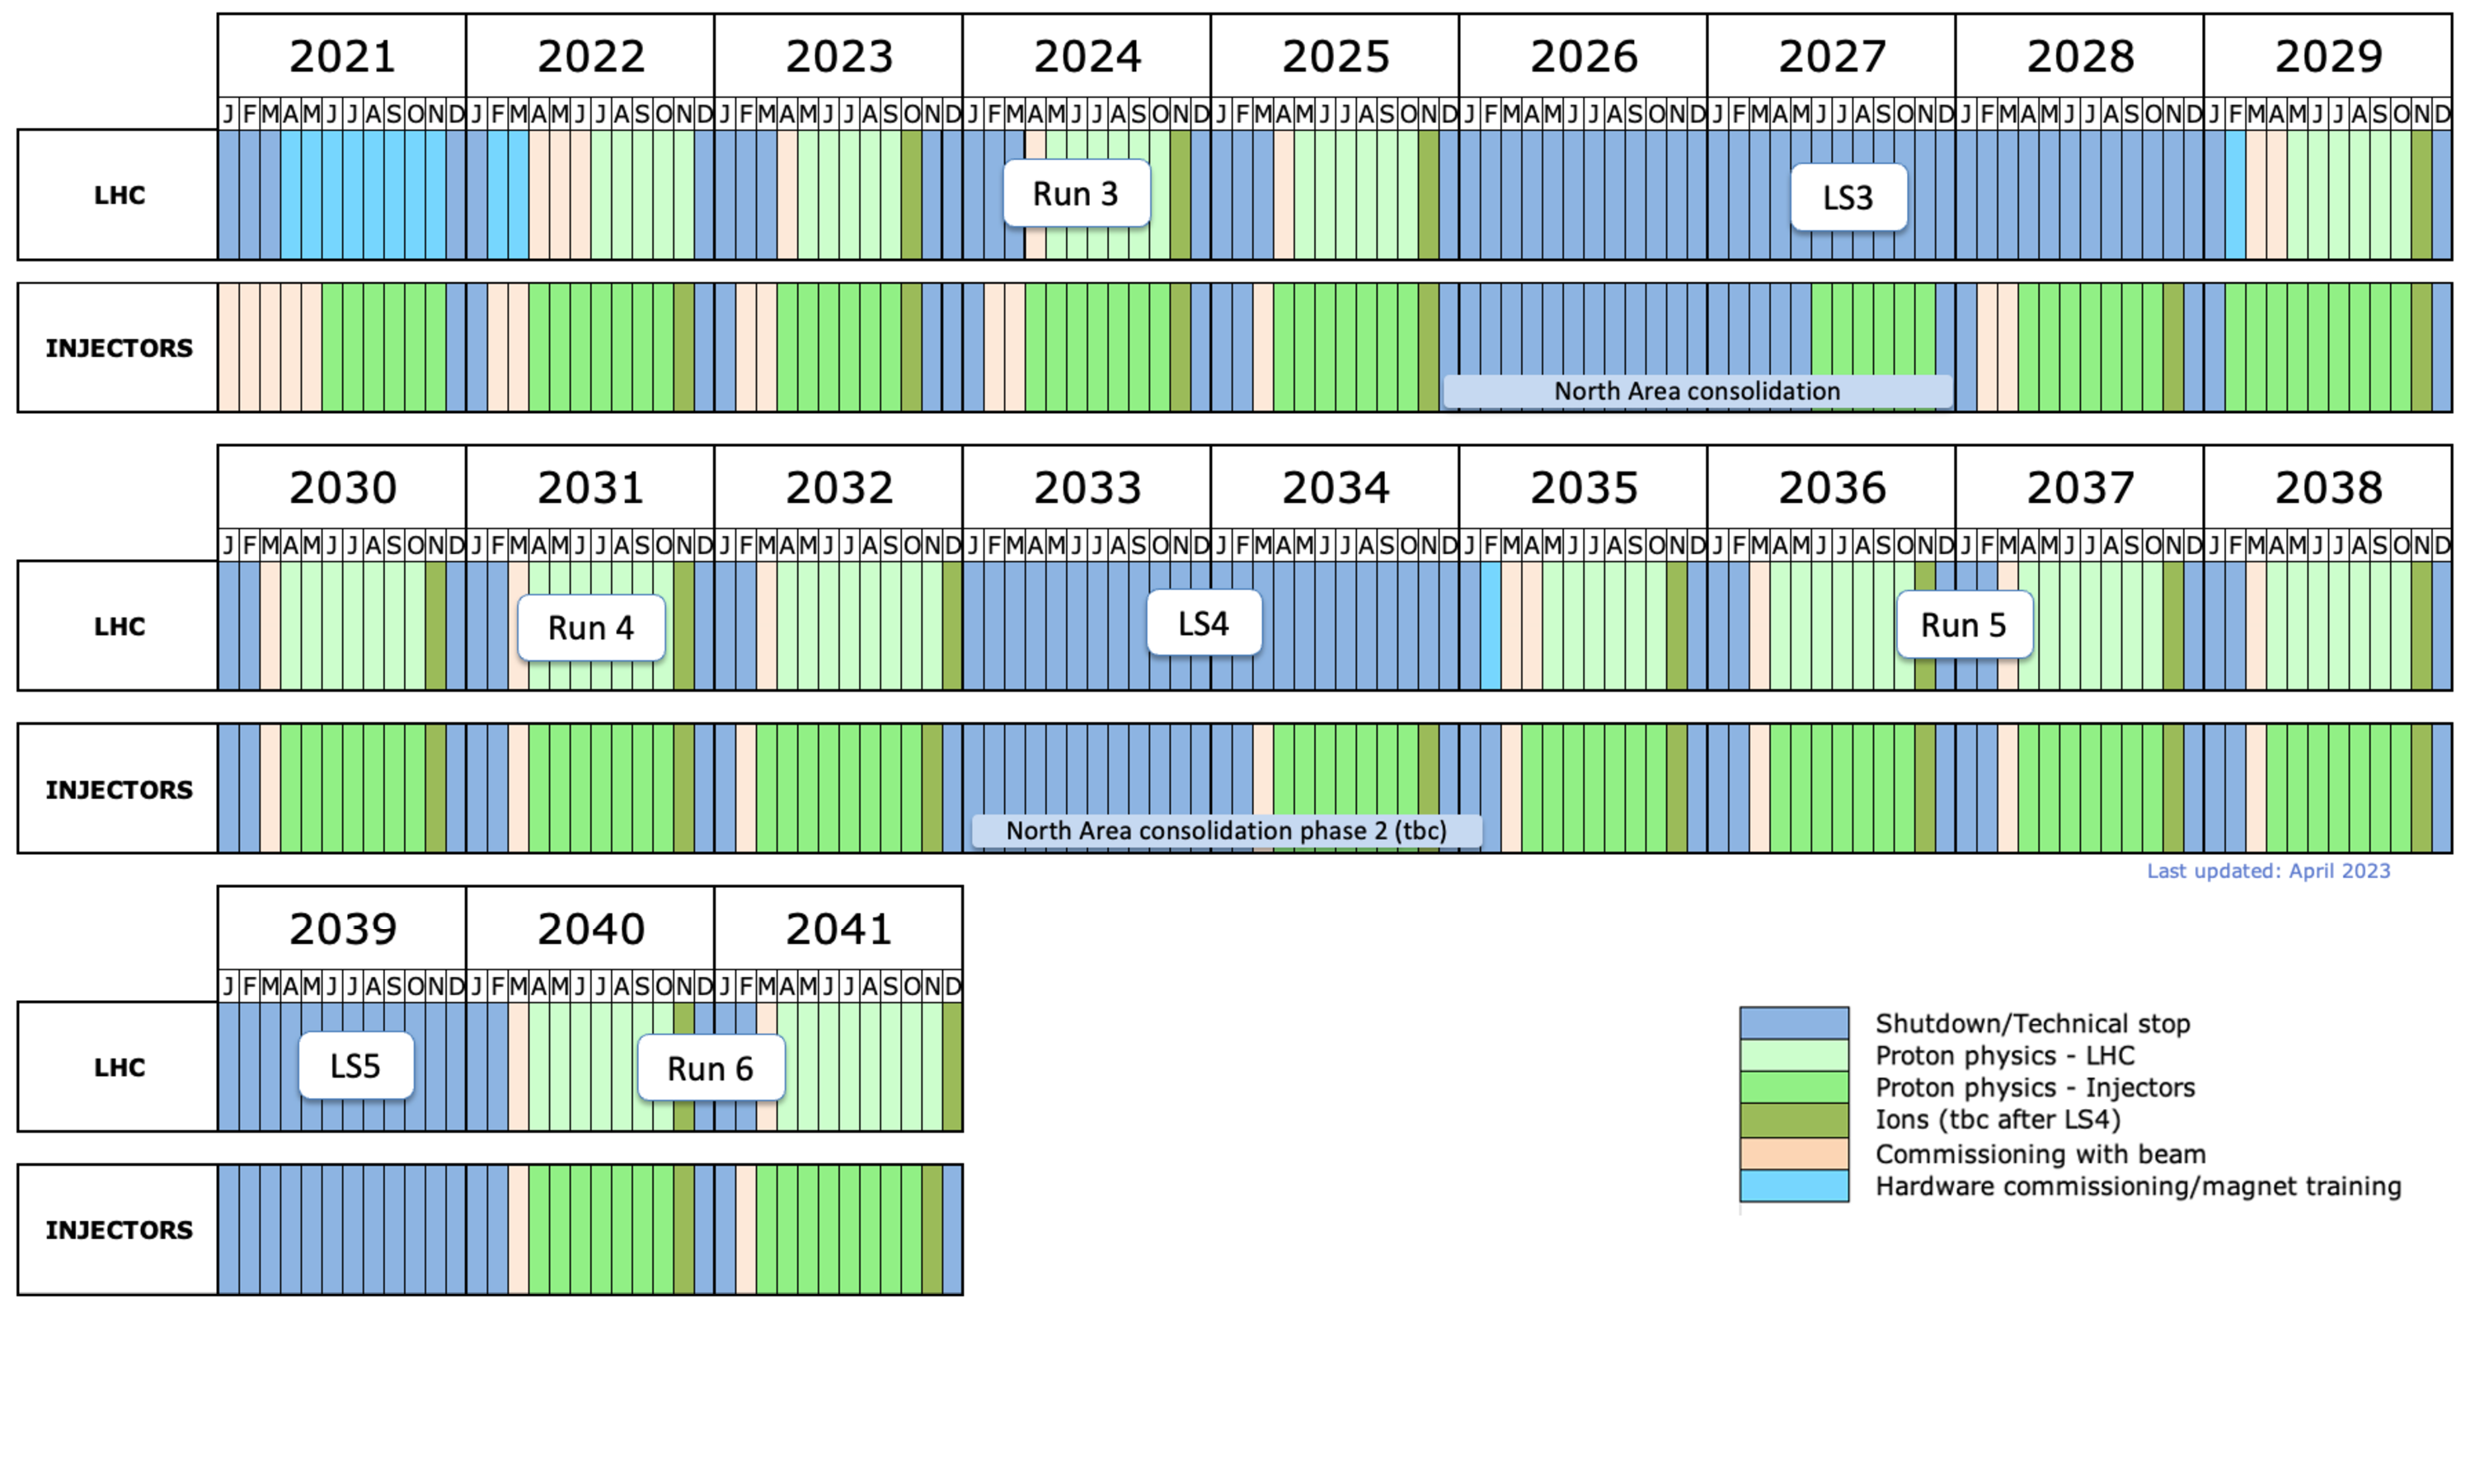
\includegraphics[width=\textwidth]{figures/Part2/LHC/Schedule}
 \end{tabular}
 \caption{The long term schedule of the \ac{LHC}, taken from~\cite{LHC:plan} in November 2023.}
 \label{fig:Schedule}
 \end{center}
\end{figure}